\providecommand{\main}{../..}

\documentclass[../../thesis]{subfiles}


\begin{document}


\chapter{Thiết kế}\label{chap:design}

Chương này tập trung vào thiết kế của ứng dụng, là triển khai cụ thể của
\autoref{chap:requirements}.

\begin{figure}[H]
    \centering
    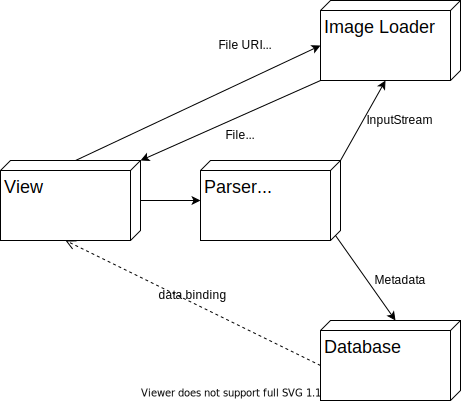
\includegraphics[width=0.6\linewidth]{../images/overall_architecture.pdf}
    \caption{Kiến trúc tổng quan của ứng dụng}
    \label{fig:overall-architecture}
\end{figure}

Kiến trúc tổng quan của yacv rất đơn giản, gồm 4 module như hình:

\begin{enumerate}
    \item
        yacv \emph{quét} metadata tệp truyện bằng module \textbf{Parser \&
        Scanner} và lưu kết quả quét vào \emph{cơ sở dữ liệu}, tức module
        \textbf{Database}
    \item
        Các \emph{Màn hình} trong module \textbf{View} hiển thị dữ liệu cho
        người dùng
    \item
        Khi người dùng đọc truyện, yacv trích xuất và lưu đệm tệp ảnh bằng
        module \textbf{Image Loader}
    \item
        Khi người dùng xem metadata, yacv trích xuất và hiển thị thông tin tệp
        truyện lên Màn hình bằng data binding với module \textbf{Database}
\end{enumerate}

Ở \fullref{chap:fundamental}, trong phần về MVVM, yacv được giới thiệu là có sử
dụng kiến trúc này. Tuy nhiên, MVVM chỉ là một phần nhỏ của ứng dụng, chủ yếu
liên quan đến việc hiển thị dữ liệu nên chỉ có ý nghĩa khi xét đến các thành
phần trong module \textbf{View}.

Ở \autoref{chap:requirements}, yêu cầu về tránh trói buộc người dùng được nên
lên đầu tiên trong các yêu cầu phi chức năng. Ở chương này, yêu cầu đó được hiện
thực hóa bằng việc \emph{yacv dùng phân vùng bộ nhớ chung}.

\begin{itemize}
    \item
        Nếu dùng phân vùng bộ nhớ riêng, yacv phải chép các tệp truyện vào đó
        (tốn thời gian và dung lượng), hơn nữa các ứng dụng đọc truyện khác
        không thể thấy được tệp truyện ở khu vực này. Tuy nhiên, dữ liệu lưu ở
        phân vùng này có thể truy cập bằng API File của Java, giúp đơn giản đáng
        kể thiết kế ứng dụng.
    \item
        Dùng phân vùng bộ nhớ chung tránh được mọi điều trên, không buộc người
        dùng vào ứng dụng, tuy nhiên lại bị giới hạn chỉ được dùng API SAF.
\end{itemize}

yacv chỉ thiết kế cho \emph{một người dùng}, do đó có rất ít tương tác, dẫn đến
kiến trúc tối giản và rời rạc như trên. Các tiểu mục sau sẽ đi sâu vào các
module này.


%----------------------------------------------------------------------------------------
%	4.1: Module Database
%----------------------------------------------------------------------------------------

% 4_1 instead of 4.1 because:
% - Maybe makeglossary doesn't recognize file with dot in name
% - This rule in .gitignore
%   *.[1-9]
\subfile{sections/section_4_1/section_4_1}


%----------------------------------------------------------------------------------------
%	4.2: Module View
%----------------------------------------------------------------------------------------

\subfile{sections/section_4_2/section_4_2}


%----------------------------------------------------------------------------------------
%	4.3: Module Parser & Scanner
%----------------------------------------------------------------------------------------

\subfile{sections/section_4_3/section_4_3}


%----------------------------------------------------------------------------------------
%	4.4: Module Image Loader
%----------------------------------------------------------------------------------------

\subfile{sections/section_4_4/section_4_4}

\end{document}
